%
% teil3.tex -- Beispiel-File für Teil 3
%
% (c) 2020 Prof Dr Andreas Müller, Hochschule Rapperswil
%
% !TEX root = ../../buch.tex
% !TEX encoding = UTF-8
%
\section{Experiment\label{kettenlinie:section:Experiment}}
\kopfrechts{Experiment}
Im Rahmen dieser Seminararbeit wurde ein Experiment durchgeführt, um das Verhalten der Kettenlinie in verschiedenen Szenarien zu veranschaulichen und ebenfalls um die hergeleiteten Formeln physikalisch zu bestätigen.

In diesem Abschnitt werden verschiedene Kettenlinien miteinander verglichen.
Ziel ist es zu beweisen, dass die Form der Kettenlinie einzig von den zwei Aufhängepunkten und der Länge der Kette selber abhängig ist.
So werden in den folgenden Versuchen immer gleich lange Ketten verwendet und an den selben Aufhängepunkten verglichen.

\subsection{Versuch 1: Kettenlinien aus verschiedenen Materialien
\label{kettenlinie:subsection:massendichte}}
\begin{figure}
	\centering
	\begin{subfigure}{0.5\textwidth}
		\centering
		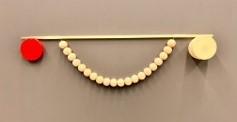
\includegraphics[width=1\textwidth]{papers/kettenlinie/images/kettenlinie_holz.jpg}
		\caption{Kette aus Holz}
		\label{fig:kettenlinie-materialien-holz}
	\end{subfigure}\hfill
	\begin{subfigure}{0.5\textwidth}
		\centering
		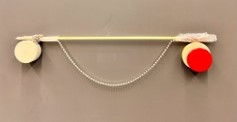
\includegraphics[width=1\textwidth]{papers/kettenlinie/images/kettenlinie_metall.jpg}
		\caption{Kette aus Metall}
		\label{fig:kettenlinie-materialien-metall}
	\end{subfigure}
	\caption{Kettenlinie für Ketten aus verschiedenen Materialien
	\label{fig:kettenlinie-materialien}}
\end{figure}
%
\begin{figure}
	\centering
	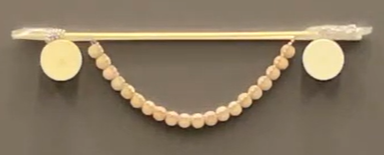
\includegraphics[width=1\textwidth]{papers/kettenlinie/images/kettenlinie_holz_metall.png}
	\caption{Holz-Kettenlinie und Metall-Kettenlinie übereinander gelegt}
	\label{fig:Kettenlinie-Holz-Metall}
\end{figure}
%
Im Abschnitt \ref{kettenlinie:subsection:Minimum der potentiellen Energie} wird hergeleitet, dass die Massendichte ignoriert werden kann. Daraus lässt sich schliessen, dass das Material, aus dem die Kette gefertigt ist, keinen Einfluss auf die Kettenlinie hat.

In den Abbildungen \ref{fig:kettenlinie-materialien}~(a) und
\ref{fig:kettenlinie-materialien}~(b) sind zwei Ketten mit derselben
Länge an zwei Aufhängepunkten mit der gleichen Distanz abgebildet.
Einziger Unterschied sind die verwendeten Materialien.
Die Kette in \ref{fig:kettenlinie-materialien}~(a) ist aus Holzperlen,
wobei in \ref{fig:kettenlinie-materialien}~(b) Metallperlen verwendet
wurden.
Metall und Holz haben eine unterschiedliche Dichte, dennoch ist die
Form der Kettenlinie für beide Ketten immer noch dieselbe, wie in
Abbildung \ref{fig:Kettenlinie-Holz-Metall} zu sehen, wo die beiden
Ketten übereinander gelegt sind.
\index{Metall}%
\index{Holz}%


\subsection{Versuch 2: Kettenlinien in verschiedenen Umgebungen
\label{kettenlinie:subsection:umgebung}}
\begin{figure}
	\centering
	\def\h{2.6}
	\def\w{3.2}
	\def\s{0.2}
	\def\t{0.2}
	\begin{subfigure}{0.50\textwidth}
		\centering
		\begin{tikzpicture}[>=latex,thick]
			\fill[color=white] (-\w,-\h) rectangle (\h,\h);
			\clip ({-\w+\s},{-\h+\t}) rectangle ({\w-\s},{\h-\t});
			\node at (0,0) {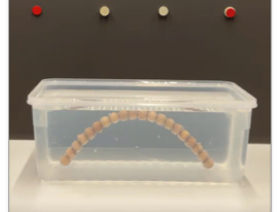
\includegraphics[width=6.4cm]{papers/kettenlinie/images/kettenlinie_holz_wasser.png}};
		\end{tikzpicture}
		\caption{Kette aus Holz im Wasser}
		\label{fig:Kettenlinie-Holz-Wasser}
	\end{subfigure}\hfill
	\begin{subfigure}{0.50\textwidth}
		\centering
		\begin{tikzpicture}[>=latex,thick]
			\fill[color=white] (-\w,-\h) rectangle (\h,\h);
			\clip ({-\w+\s},{-\h+\t}) rectangle ({\w-\s},{\h-\t});
			\node at (0,0) {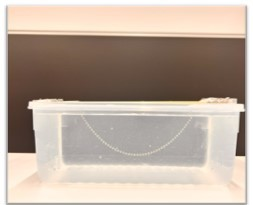
\includegraphics[width=6.4cm]{papers/kettenlinie/images/kettenlinie_metall_wasser.jpg}};
		\end{tikzpicture}
		\caption{Kette aus Metall im Wasser}
		\label{fig:Kettenlinie-Metall-Wasser}
	\end{subfigure}
	\caption{Ketten unter Wasser ergeben die gleiche Kettenlinie unabhängig
	vom Material.
	\label{fig:kettenlinie-wasser}}
\end{figure}
%
\begin{figure}
	\centering
	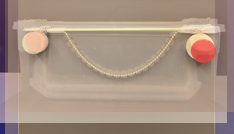
\includegraphics[width=1\textwidth]{papers/kettenlinie/images/kettenlinie_merged.png}
	\caption{Vier Kettenlinien übereinander gelegt}
	\label{fig:Kettenlinie-Merged}
\end{figure}
%
Auch in Abschnitt \ref{kettenlinie:subsection:Minimum der potentiellen Energie} wird die Gravitationskonstante ignoriert.
Da die Gravitation keine Rolle spielt für die Form der Kettenlinie, lässt sich annehmen dass egal in welcher Umgebung die Kette aufgehängt wird, sie immer in derselben Form bleibt.
Wichtig ist nur, dass eine Gravitationskraft existiert.
Um diese Annahme zu testen, werden die Kettenlinien von Versuch 1 im Abschnitt \ref{kettenlinie:subsection:massendichte} wiederverwendet, aber diesmal in Wasser aufgehängt.

In den Abbildungen \ref{fig:kettenlinie-wasser}~(a) und
\ref{fig:kettenlinie-wasser}~(b) sind diese Kettenlinien im Wasser zu sehen.
Legt man diese wieder übereinander, sieht man dass die Form unverändert bleibt.
In Abbildung \ref{fig:Kettenlinie-Merged} wird dies, zusätzlich mit den Kettenlinien aus Versuch 1, nochmal veranschaulicht.

\subsection{Versuch 3: Kettenlinien im Wasser
\label{kettenlinie:subsection:wasser}}

Aus dem vorherigen Versuch, wurden einige Verhaltensänderungen festgestellt.
So entsteht bei der Kette aus Holz eine umgekehrte Kettenlinie im Wasser.
Grund dafür ist natürlich die geringere Dichte von Holz gegenüber von Wasser.
Da die Aufhängepunkte der Kette unter Wasser sind, entsteht durch den Auftrieb eine umgekehrte Kettenlinie.
Diese Kettenlinie hat immer noch dieselbe Form wie die restlichen Kettenlinien in diesem Experiment, jedoch um 180° gedreht.

In der Abbildung \ref{fig:Kettenlinie-Curves} ist eine weitere Besonderheit zu sehen.
\begin{figure}
	\centering
	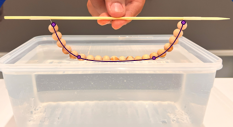
\includegraphics[width=1\textwidth]{papers/kettenlinie/images/kettenlinie_curves.png}
	\caption{Kettenlinie mit Knicke, es entstehen drei Kettenlinien}
	\label{fig:Kettenlinie-Curves}
\end{figure}

Wenn die Holzkettenlinie auf der Wasseroberfläche aufkommt, entstehen durch den Auftrieb Knicke.
Spannend dabei ist, dass dadurch drei Segmente entstehen.
In jedem Segment entsteht zwischen den Knicken eine eigene, neue Kettenlinie.


\subsection{Fazit Experiment
\label{kettenlinie:subsection:fazit-experiment}}
Aus dem Experiment ist klar erkennbar, dass Faktoren wie Materialdichte und Gravitationskräfte keine Auswirkungen auf die Form der jeweiligen Kettenlinie haben.
Die mathematischen Herleitungen stimmen und wurden durch die Experimente auch visuell bewiesen.
